\documentclass[runningheads]{llncs}

\usepackage{graphicx}
\usepackage{multirow}


\begin{document}

\title{YOLOv4 and how one-stage detectors may take over two-stage detectors}


\author{Joris LIMONIER}

\authorrunning{J. LIMONIER}

\institute{University of Côte d'Azur
    \email{joris.limonier@hotmail.fr}
    % \url{https://www.linkedin.com/in/joris-limonier-a48a0213a/}
}

\maketitle

% Title
% Authors
% Abstract
% SOTA
% Discussion
% Conclusion

\begin{abstract}
    In the last 20 years, the field of object detection has become more and more prevalent. With Viola \& Jones (2001), the field started with traditional methods. From 2014 on, more modern Deep Learning techniques were adopted, which lead to two main types of detectors: One-stage detectors and Two-stage detectors. In this paper we focus on the former, more particularly on YOLOv4 (You Only Look Once), and we compare it to the latter. One-stage detectors are meant to focus on speed of execution, while trying to keep a decent accuracy. Today, their accuracy still lacks behind the one of two-stage detectors in some cases, but their fast improvement makes us wonder whether they will take over two-stage detectors. In particular, YOLOv4 represents a great improvement over previous recent methods, showing impressive results both in accuracy and in speed.

    \keywords{YOLOv4 \and Object detection \and One-stage detectors \and Two-stage detectors}
\end{abstract}

\section{State of the Art}
As shown in figure \ref{fig: evolution of publications}, the number of object detection-related publications per year has been greatly increasing over the past 20 years \cite{zou_object_2019}. As a result, many detectors are now available for comparison with the one we are interested in, YOLOv4.

\begin{figure}
    \centering
    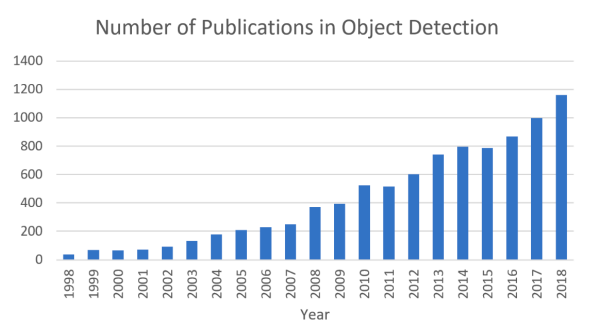
\includegraphics[width=.7\textwidth]{media/number_publications.png}
    \caption{Number of publications per year between 1998 and 2018 in the field of object detection.}
    \label{fig: evolution of publications}
\end{figure}

Figure \ref{fig: SOTA comparison} compares YOLOv4 to several of the most recent contenders, namely: YOLOv3 \cite{redmon_yolov3_2018}, EfficientDet \cite{tan_efficientdet_2020}, Adaptive Training Sample Selection (ATSS) \cite{zhang_bridging_2020}, Adaptively Spatial Feature Fusion (ASFF) \cite{liu_learning_2019} and CenterMask \cite{lee_centermask_2020}.

\begin{figure}
    \centering
    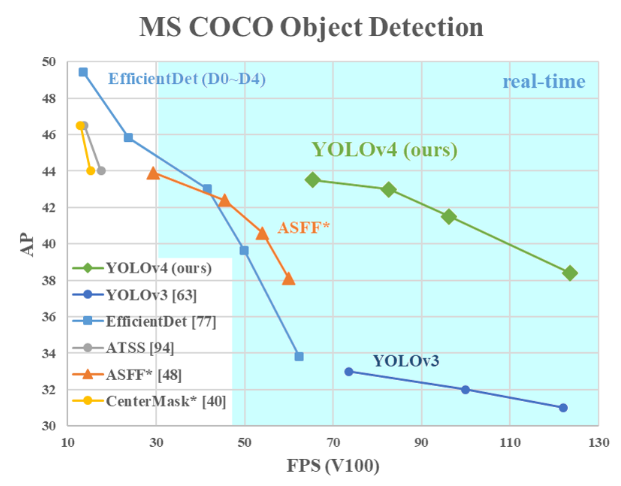
\includegraphics[width=.7\textwidth]{media/YOLO_performance_comparison.png}
    \caption{Comparison between YOLOv4 and several other state of the art object detectors on the COCO dataset. This figure comes from Bochkovskiy et al. \cite{bochkovskiy_yolov4_2020} and the numbers in the caption refer to their references.}
    \label{fig: SOTA comparison}
\end{figure}

Except for YOLOv3, it appears in figure \ref{fig: SOTA comparison} that for a given speed, YOLOv4 is more accurate than all other state of the art (SOTA) methods, and given an accuracy, YOLOv4 is faster than all other SOTA methods. When compared to its predecessor (YOLOv3), figure \ref{fig: SOTA comparison} doesn't show improvements in speed (not measured), but a great step forward in terms of accuracy. The accuracy improvement is fairly substantial, with an increase of about 30\% in prediction correctness (from 32\% to 42\%). Moreover, the two papers have only been published two years apart from one another.


\section{Discussion and conclusion}
As mentioned previously, there are two types of object detectors: one-stage detectors and two-stage detectors. The former focus on speed and are capable of directly detecting objects without a preliminary steps. The latter are usually more accurate but they need a preliminary step in order to determine regions of interest and before classifying them. \\
YOLOv4 is a one-stage object detector, but as shown in table \ref{table: comparison in accuracy between one- and two-stage SOTA detectors}, it performs similarly, or even higher, than other SOTA two-stage detectors ($38.4\% - 43.0\%$ against $43.0\%$ for YOLOv4). The numbers have been gathered from two sources however: the accuracy for YOLOv4 comes from Bochkovskiy et al. \cite{bochkovskiy_yolov4_2020}, whereas the other accuracies come from Carranza-Garcia et al. \cite{carranza-garcia_performance_2020} so despite our efforts to compare apples to apples, some disparities in the computation of the accuracy may have gone through. As a results, it seems fair to state that YOLOv4 performs ``at least as well'' as the other two-stage detectors measured. Therefore, based on the observations from \ref{table: comparison in accuracy between one- and two-stage SOTA detectors}, it appears that YOLOv4 doesn't perform worse than two-stage detectors, while showing more attractive classification speeds. \\

\begin{table}
    \centering
    \caption{Comparison in accuracy between SOTA two-stage detectors (using Faster RCNN) and one-stage detectors on the COCO dataset.}
    \begin{tabular}{c|c|c|c}
         & \textbf{Architecture} & \textbf{Feature extractor} & \textbf{Accuracy (\%)} \\
        \hline
        \multirow{5}{*}{\textbf{Two-stage detectors}}
         & Faster RCNN           & FPN Res2Net101             & $43.0$                 \\
         & Faster RCNN           & FPN ResNeXt101             & $41.2$                 \\
         & Faster RCNN           & FPN ResNet152              & $40.1$                 \\
         & Faster RCNN           & FPN ResNet101              & $39.8$                 \\
         & Faster RCNN           & FPN ResNet50               & $38.4$                 \\
        \hline
        \multirow{2}{*}{\textbf{One-stage detectors}}
         & YOLOv3                & DarkNet-53                 & $33.4$                 \\
         & YOLOv4                & CSPDarknet-53              & $43.0$
    \end{tabular}
    \label{table: comparison in accuracy between one- and two-stage SOTA detectors}
\end{table}

So what are the advantages of two-stage detectors ? Object recognition is making its way into more and more devices around us. These devices often strongly rely on fast identification of what is coming through video input (\textit{e.g.} self-driving cars). Other devices require reliable identification given little computing power (\textit{e.g.} robot vacuum cleaners), which goes alongside faster classification speeds. \\
Furthermore, the rate of improvement shown in figure \ref{fig: SOTA comparison} and table \ref{table: comparison in accuracy between one- and two-stage SOTA detectors} between YOLOv3 and YOLOv4 in only two years time hints that even more impressive results could be obtained in the upcoming years. A similar trend would allow the elaboration of significantly faster and more accurate detectors in the near future. By continuing on a similar progression, it seems that one-stage detectors could make two-stage detectors obsolete rather sooner than later. \\
It appears to us that one-stage detectors may be the way to go and will probably take over the majority of cases of object detection. A word of caution however, in the case of slow processes (not heavily time reliant), it is possible that two-stage detectors may still remain in use. Such cases may value accuracy much more than they value speed, therefore preferring those longer detectors. Additionally, Carranza-Garcia et al. \cite{carranza-garcia_performance_2020} also bring proof of some specific cases where two-stage detectors perform better than their counterpart, such as high resolution. Indeed, although the accuracy is comparable between the two type of detectors in low-resolution images ($\approx 42\%$ against $\approx 45\%$), the gap widens for high-resolution images ($\approx 48\%$ against $\approx 56\%$). \\
So the only question remaining is whether one-stage detectors will become absolutely more accurate (that is, not relatively to speed but simply beating two-stage detectors in terms of accuracy). Our prediction on that front is that \textbf{they will}, however this will probably still take a couple years, or even decades. The dynamic seems in favor of one-stage detectors but they still have some way to go before being completely on part with two-stage ones. They have even more way to go (if it ever happens) until systematically being superior, that is in all edge cases, for all types of objects and under all circumstances (such as the image resolution). The whole process of identifying a region of interest before clasifying objects in it seems too cumbersome to be true. Analogically, it seems like issues faced by physicists with two irreconcilable theories that one day someone manages to merge in a more elegant way. Our opinion is that the field of object detection is waiting for such a kind of event to occur and that this reunification will come eventually.

\bibliographystyle{splncs04}
\bibliography{ExportedItems}
\end{document}
